\documentclass{beamer} %[10pt,handout]
\usetheme{Copenhagen}
\usecolortheme{rose}
\usepackage{showexpl, graphicx, booktabs, tikz,tikzscale}
\usepackage[xspace]{ellipsis}
\usepackage{fancyvrb}

% This automatically created a section slide 
\AtBeginSection[]{
  \begin{frame}
  \vfill
  \centering
  \begin{beamercolorbox}[sep=8pt,center,shadow=true,rounded=true]{title}
    \usebeamerfont{title}\insertsectionhead\par%
  \end{beamercolorbox}
  \vfill
  \end{frame}
}

%%%% Title %%%%
\title[{\LaTeX} Workshop] % (optional, only for long titles)
{{\LaTeX}  Workshop}
\subtitle{}
\author[Therese Anders] % (optional, for multiple authors)
{Therese Anders\inst{1}}
\institute[] % (optional)
{
  \inst{1}%
  PhD Candidate\\
  School of International Relations\\
  University of Southern California
}
\date[7 February 2018] % (optional)
{7 February 2018}
\subject{Conflict and Government Investment}

%%%% Start of Presentation %%%%
\begin{document}

\frame{\titlepage}

%%% INTRO


\begin{frame}
\frametitle{Plan for the Workshop}
\begin{enumerate}
\item Introduction. \hyperlink{intro}{\beamerbutton{$\rightarrow$}}
\item Why bother learning {\LaTeX}? \hyperlink{why}{\beamerbutton{$\rightarrow$}}
\item Challenges and downsides. \hyperlink{challenge}{\beamerbutton{$\rightarrow$}}
\item Basic structure of a {\LaTeX} document and compiling.  \hyperlink{structure}{\beamerbutton{$\rightarrow$}}
\item Bibliographies.\hyperlink{bib}{\beamerbutton{$\rightarrow$}}
\item Article-style document: Formatting, figures, tables, bibliographies, equations (accompanying template).
\end{enumerate}
\end{frame}

\section{Introduction}\label{intro}
 
 \begin{frame}
 \frametitle{What is {\LaTeX?}}
 {\LaTeX} is a typesetting language that allows you to produce publication-ready documents.
 \end{frame}
 
\begin{frame}
\frametitle{Goal for this Workshop}
Give you a jump start into working with {\LaTeX}.  \pause
\begin{block}{Key to learning {\LaTeX}}
{\begin{itemize}
\item<1-> Good template.
\item<2-> Basic idea of the structure of  {\LaTeX} documents.
\item<3-> Google should be your bff.
\item<4-> Willingness to suffer a bit in the beginning.
\end{itemize}}
\end{block}
\end{frame}
 
 \begin{frame}
\frametitle{Friendly Warning}
If your dissertation is due in 2 weeks, {\Huge\underline{do not}} start typesetting it in {\LaTeX} now!
\end{frame}
 
 %%% WHY
\section{Why bother learning {\LaTeX}}\label{why}

\begin{frame}
\frametitle{Just a few reasons why you should be using \LaTeX}
\begin{itemize}
\item<1-> Free, open source.
\item<2-> Beautiful typesetting.
\item<3-> Inserting and updating tables/figures from \texttt{R} or Stata.
\item<4-> Inserting/updating bibliographies.
\item<5-> Math typesetting and formal presentation (game trees, diagrams). 
\end{itemize}
\end{frame}

%%
\subsection{Typography}

%\begin{frame}
%\frametitle{{\LaTeX} uses an advanced typesetting algorithm}
%\begin{figure}[htbp]
%\begin{center}
%
\includegraphics[width = 1.7in]{latex_comic.jpg}
%\caption{\scriptsize Source \url{http://bit.ly/25VwZaG}.}
%\end{center}
%\end{figure}
%\end{frame}

\begin{frame}
\Huge\centering
\LaTeX---The quiz!
\end{frame}
 
 %Articles
\begin{frame}
\frametitle{The Quiz: {\LaTeX} or Word?}
\begin{figure}[htbp]
\begin{center}
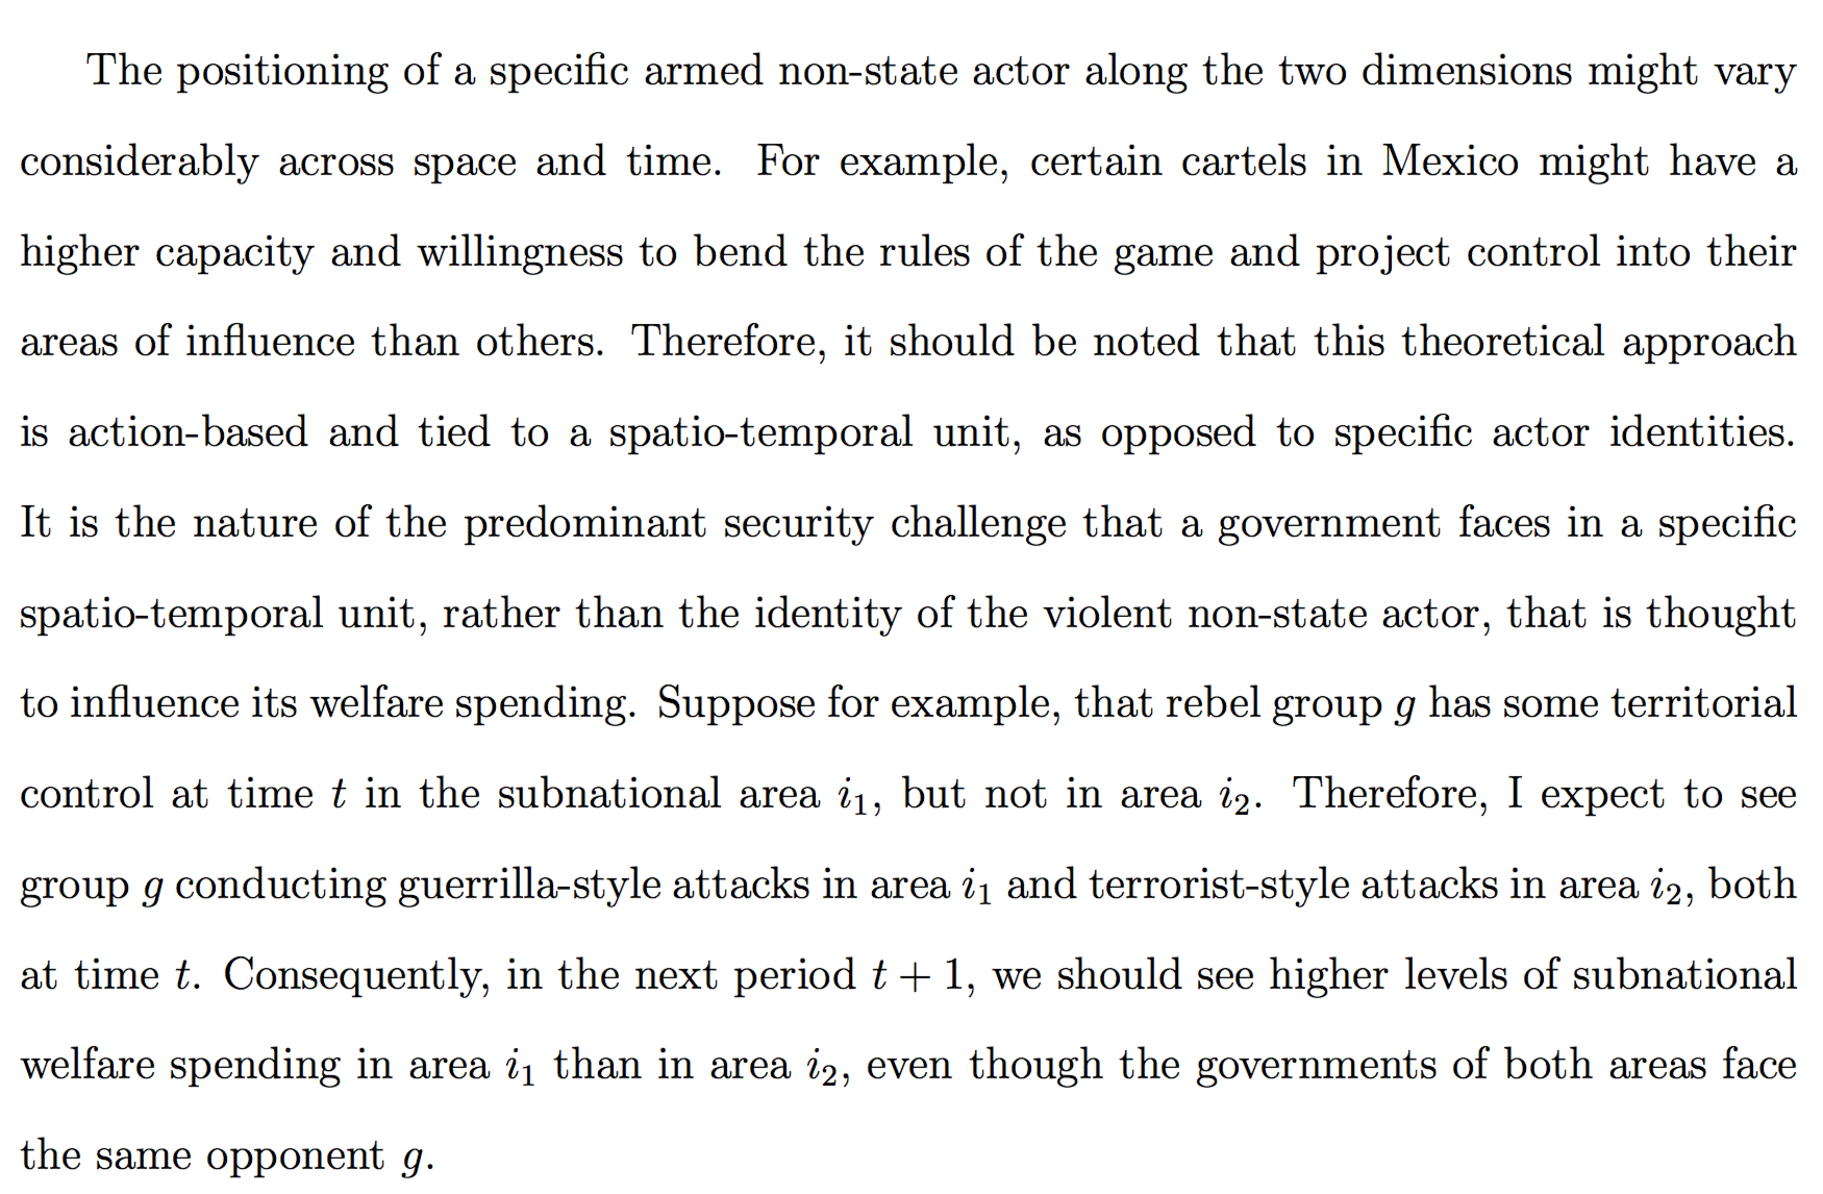
\includegraphics[width = 3.5in]{latex1.pdf}
\end{center}
\end{figure}
\end{frame}

\begin{frame}
\frametitle{The Quiz: {\LaTeX} or Word?}
\begin{figure}[htbp]
\begin{center}
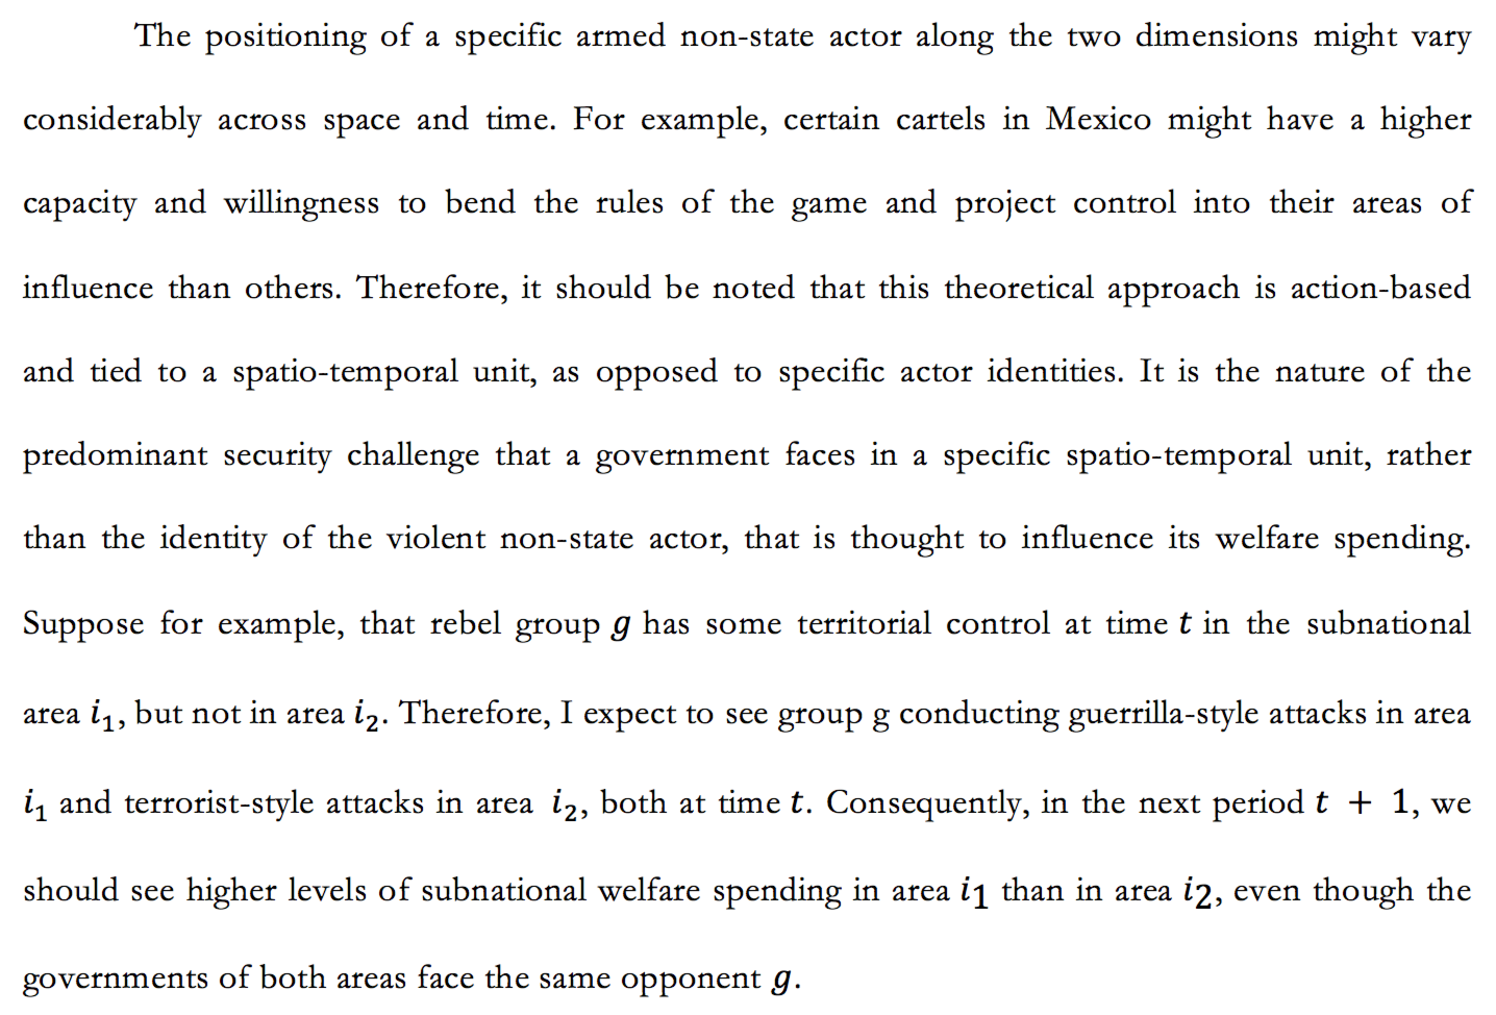
\includegraphics[width = 3.5in]{word1.pdf}
\end{center}
\end{figure}
\end{frame}
 
%Lists
\begin{frame}
\frametitle{The Quiz: {\LaTeX} or Word?}
\begin{figure}[htbp]
\begin{center}
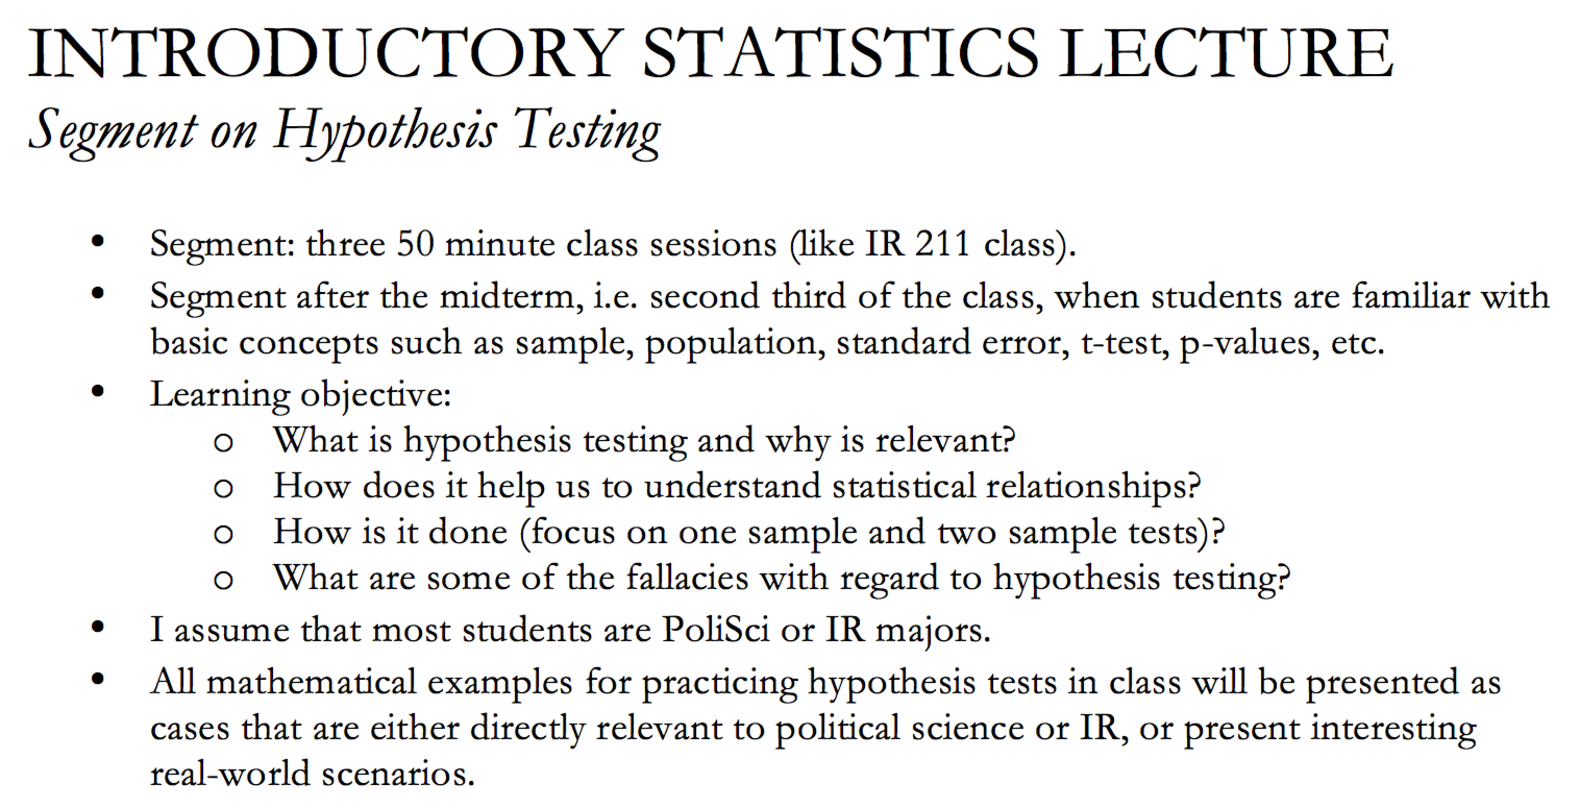
\includegraphics[width = 4in]{word2.pdf}
\end{center}
\end{figure}
\end{frame}

\begin{frame}
\frametitle{The Quiz: {\LaTeX} or Word?}
\begin{figure}[htbp]
\begin{center}
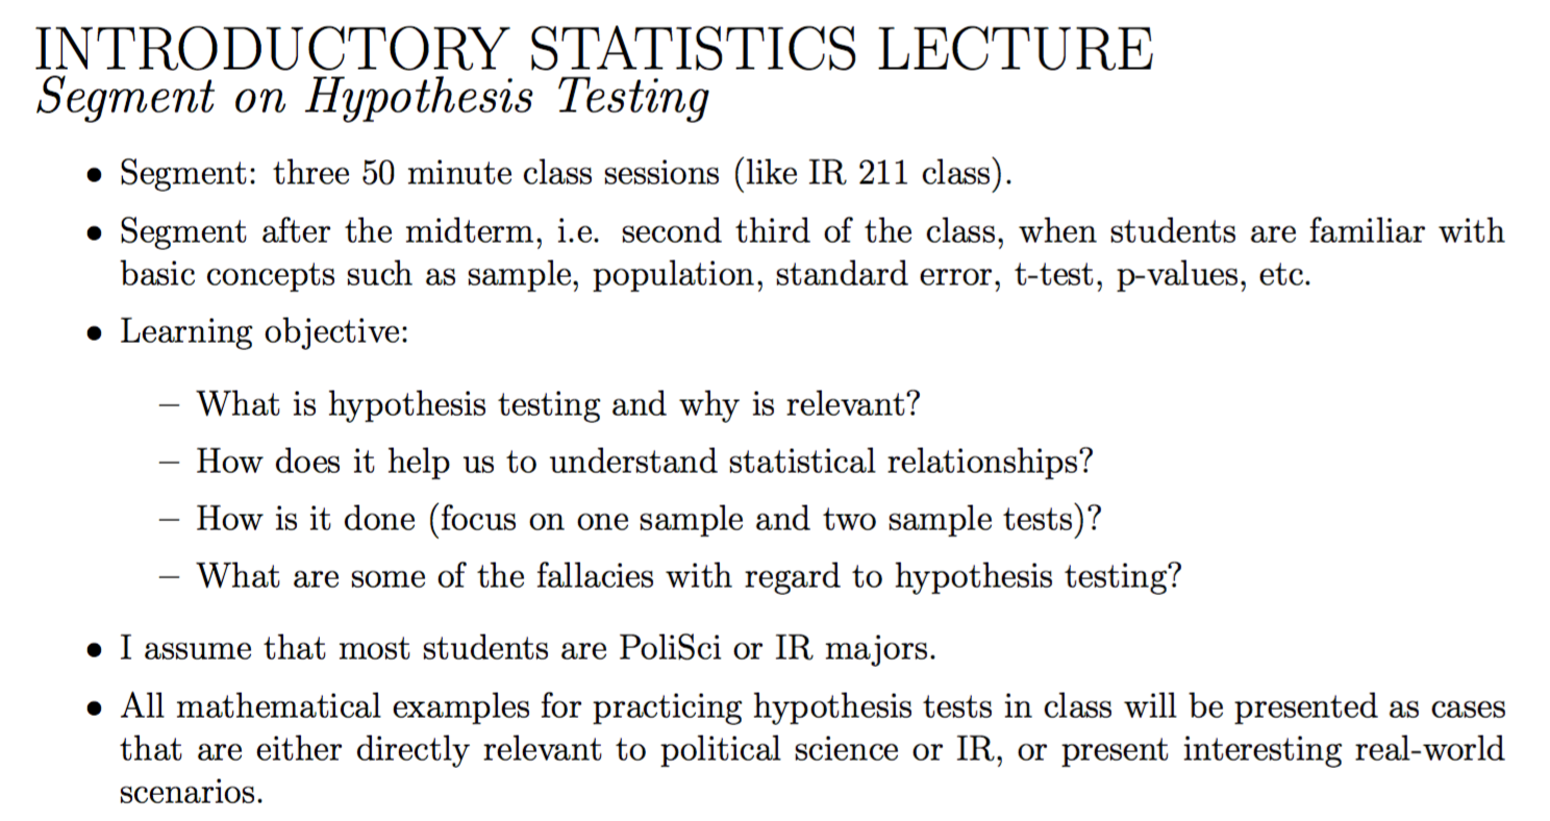
\includegraphics[width = 4in]{latex2.pdf}
\end{center}
\end{figure}
\end{frame}


\begin{frame}
\frametitle{The Quiz: {\LaTeX} or Word?}
\begin{figure}[htbp]
\begin{center}
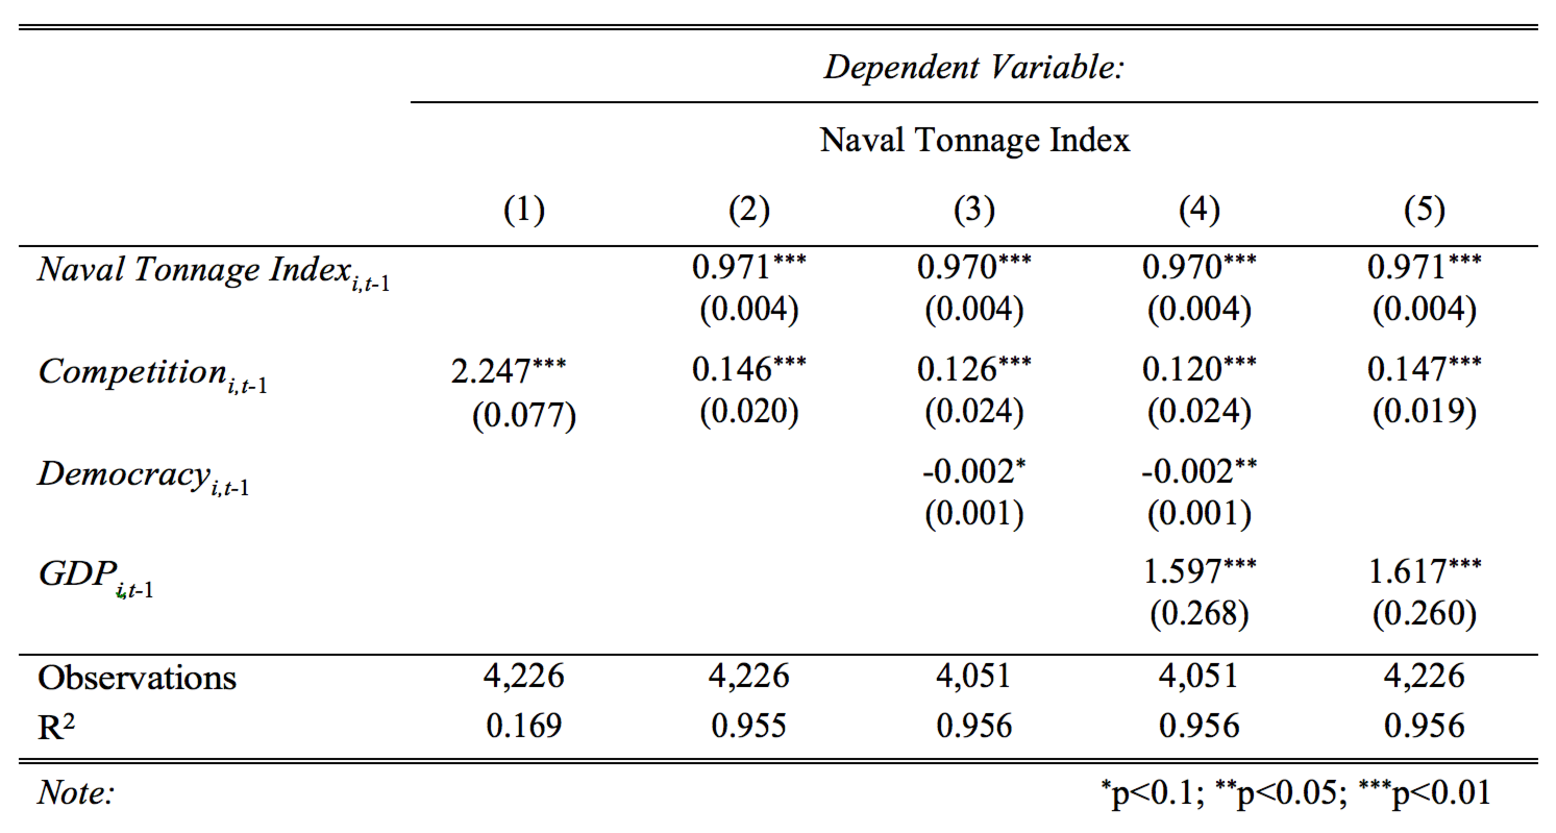
\includegraphics[width = 3in]{word3.pdf}
\caption{\tiny Markowitz, J. and C. Fariss: Power, Proximity, and Democracy: Geopolitical Competition in the International System. In \textit{Journal of Peace Research} (Forthcoming).}
\end{center}
\end{figure}
\end{frame}

\begin{frame}
\frametitle{The Quiz: {\LaTeX} or Word?}
\begin{figure}[htbp]
\begin{center}
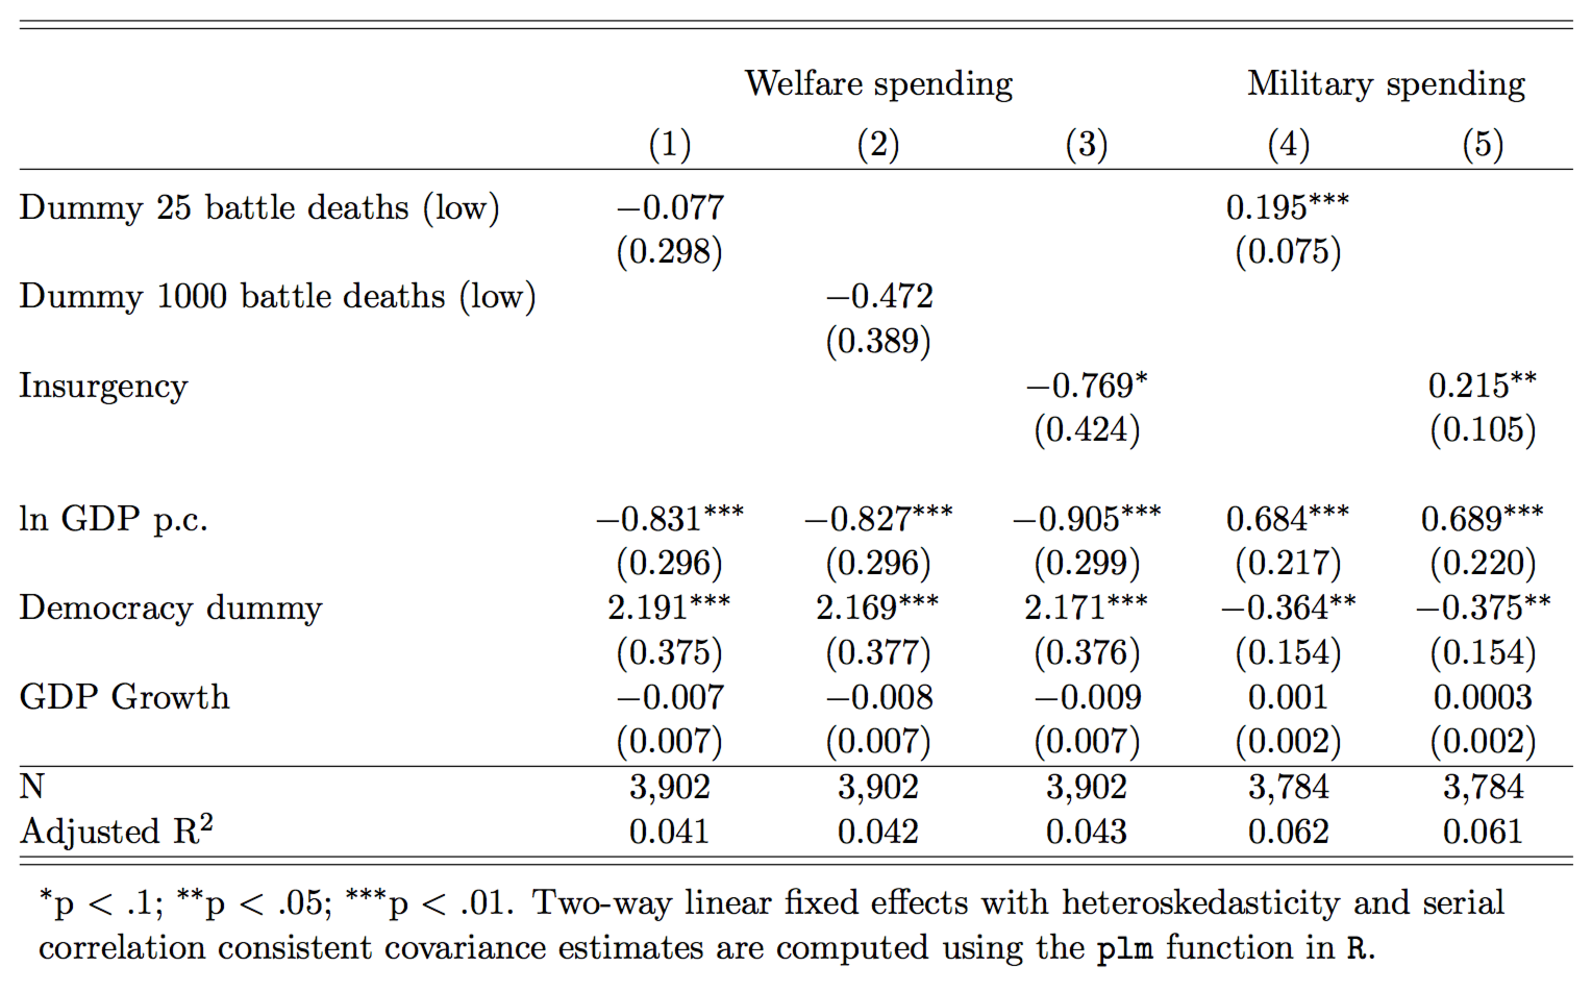
\includegraphics[width = 3in]{latex3.pdf}
\caption{\tiny Anders, T. \textit{The Relationship Between Violent Conflict and Welfare Spending Revisited} (unpublished manuscript).}
\end{center}
\end{figure}
\end{frame}
 
%\begin{frame}
%\frametitle{Comparing Word, InDesign, and {\LaTeX}}
%	\begin{figure}[htbp]
%	\begin{center}
%	\includegraphics[width = 3.8in]{comparison.pdf}
%	\caption{\url{http://www.zinktypografie.nl/comparison.pdf}.}
%	\end{center}
%	\end{figure}
%\end{frame}
 
%\begin{frame}
%\frametitle{Comparing Word, InDesign, and {LaTeX}}
%	\begin{figure}[htbp]
%	\begin{center}
%	\includegraphics[width = 4in]{comparison_table.pdf}
%	\caption{\url{http://www.zinktypografie.nl/comparison.pdf}. Inter-word spacing is the spacing between words. {\LaTeX} uses an advanced algorithm to compute the optimal IWS for each document.}
%	\end{center}
%	\end{figure}
%\end{frame}
 
 %%
\subsection{Separation of content and presentation}

\begin{frame}
\frametitle{\textsc{wysiwyg} and \textsc{wysiwym}}
\begin{block}{what-you-see-is-what-you-get (\textsc{wysiwyg})}
Content $=$ presentation. Example: Word.
\end{block}
\begin{block}{  what-you-see-is-what-you-mean (\textsc{wysiwym})}
Content $\neq$ presentation. Example: {\LaTeX}.
\end{block}
\end{frame}

\begin{frame}[fragile]
\frametitle{Example for Separation of Content and Presentation}
\begin{center}
If your dissertation is due in 2 weeks, 
{\Huge\underline{do not}} start typesetting it in {\LaTeX} now!
\end{center}
\begin{scriptsize}
\begin{verbatim}
\begin{center}
If your dissertation is due in 2 weeks, 
{\Huge\underline{do not}} start typesetting it in {\LaTeX} now!
\end{center}
\end{verbatim}
\end{scriptsize}
\end{frame}
 
\begin{frame}
\frametitle{Pros and Cons: Separation of Content and Presentation}
\begin{block}{Pros}%
\begin{itemize}
\item Reproducibility.
\item Stability.
\item Unambiguous.
\item Once set up, no need to worry about formatting. In fact, you \underline{should} focus on content over form. {\LaTeX} will do the rest the form for you. $\Longrightarrow$ Templates!
\end{itemize}
\end{block}
\begin{block}{Cons}%
\begin{itemize}
\item No/few ``buttons'' to press---need to learn commands.
\item Steep learning curve. Can be time intensive.
\end{itemize}
\end{block}
\end{frame} 
 
%%
\subsection{Integration of data from other sources}

\begin{frame}
\frametitle{Working Directory (WD)}
\begin{itemize}
\item The WD is a specified path (think folder) on your machine.
\item The program will look for and store all data in the WD.
\item Unless otherwise specified, {\LaTeX} will use the folder where the main .tex file is stored as WD.
\item Store all auxiliary data (graphs, tables, etc.) in the WD.
\end{itemize}
\end{frame}

\begin{frame}[fragile=singleslide]
\frametitle{Adding graphs to {\LaTeX} files.}
\begin{Verbatim}
\begin{figure}[h!] 
\begin{center}

\includegraphics[width = 2in]{latex_comic.jpg}
\caption{Source \url{http://bit.ly/25VwZaG}.}
\label{comic_fig}
\end{center}
\end{figure}
\end{Verbatim}
\end{frame}

\begin{frame}[fragile=singleslide]
\frametitle{Integration of tables is one of the main perks!}
\begin{itemize}
\item \texttt{R} packages such as \texttt{stargazer} or \texttt{xtable} will output beautifully formatted (regression) tables as a .tex file. 
\item \texttt{estout} package for Stata.
\item Save the .tex file directly to you WD, then import the file into your {\LaTeX} document.
\end{itemize}
\end{frame}
 
\begin{frame}[fragile=singleslide]
\frametitle{\texttt{$\backslash$input\{\}} command}
The following table (\texttt{stargazer} output) is imported by the following line:
\begin{center}
\begin{verbatim}

% Table created by stargazer v.5.1 by Marek Hlavac, Harvard University. E-mail: hlavac at fas.harvard.edu
% Date and time: Wed, Apr 13, 2016 - 12:31:07
\begin{tabular}{@{\extracolsep{5pt}}lcccc} 
\\[-1.8ex]\hline 
\hline \\[-1.8ex] 
 & \multicolumn{4}{c}{\textit{Dependent variable:}} \\ 
\cline{2-5} 
\\[-1.8ex] & \multicolumn{3}{c}{internet} & life\_exp \\ 
\\[-1.8ex] & (1) & (2) & (3) & (4)\\ 
\hline \\[-1.8ex] 
 polity & 0.255$^{***}$ & 0.084$^{***}$ &  &  \\ 
  & (0.023) & (0.020) &  &  \\ 
  & & & & \\ 
 pop &  & 0.000 &  &  \\ 
  &  & (0.000) &  &  \\ 
  & & & & \\ 
 gdppc &  & 0.001$^{***}$ &  & 0.0005$^{***}$ \\ 
  &  & (0.00002) &  & (0.00001) \\ 
  & & & & \\ 
 life\_exp &  &  & 1.101$^{***}$ &  \\ 
  &  &  & (0.031) &  \\ 
  & & & & \\ 
 Constant & 15.002$^{***}$ & 5.955$^{***}$ & $-$60.212$^{***}$ & 62.576$^{***}$ \\ 
  & (0.401) & (0.408) & (2.098) & (0.160) \\ 
  & & & & \\ 
\hline \\[-1.8ex] 
Observations & 3,126 & 3,003 & 3,376 & 4,111 \\ 
R$^{2}$ & 0.039 & 0.384 & 0.276 & 0.334 \\ 
Adjusted R$^{2}$ & 0.038 & 0.383 & 0.276 & 0.334 \\ 
Residual Std. Error & 22.391 (df = 3124) & 17.953 (df = 2999) & 18.534 (df = 3374) & 8.625 (df = 4109) \\ 
F Statistic & 125.913$^{***}$ (df = 1; 3124) & 622.987$^{***}$ (df = 3; 2999) & 1,285.932$^{***}$ (df = 1; 3374) & 2,063.299$^{***}$ (df = 1; 4109) \\ 
\hline 
\hline \\[-1.8ex] 
\textit{Note:}  & \multicolumn{4}{r}{$^{*}$p$<$0.1; $^{**}$p$<$0.05; $^{***}$p$<$0.01} \\ 
\end{tabular} 

\end{verbatim}
\end{center}
 
\begin{scriptsize}
Disclaimer: In reality, to import the table into the \texttt{beamer} class, I use a  wrapper: \begin{verbatim} \resizebox{\linewidth}{!}{
% Table created by stargazer v.5.1 by Marek Hlavac, Harvard University. E-mail: hlavac at fas.harvard.edu
% Date and time: Wed, Apr 13, 2016 - 12:31:07
\begin{tabular}{@{\extracolsep{5pt}}lcccc} 
\\[-1.8ex]\hline 
\hline \\[-1.8ex] 
 & \multicolumn{4}{c}{\textit{Dependent variable:}} \\ 
\cline{2-5} 
\\[-1.8ex] & \multicolumn{3}{c}{internet} & life\_exp \\ 
\\[-1.8ex] & (1) & (2) & (3) & (4)\\ 
\hline \\[-1.8ex] 
 polity & 0.255$^{***}$ & 0.084$^{***}$ &  &  \\ 
  & (0.023) & (0.020) &  &  \\ 
  & & & & \\ 
 pop &  & 0.000 &  &  \\ 
  &  & (0.000) &  &  \\ 
  & & & & \\ 
 gdppc &  & 0.001$^{***}$ &  & 0.0005$^{***}$ \\ 
  &  & (0.00002) &  & (0.00001) \\ 
  & & & & \\ 
 life\_exp &  &  & 1.101$^{***}$ &  \\ 
  &  &  & (0.031) &  \\ 
  & & & & \\ 
 Constant & 15.002$^{***}$ & 5.955$^{***}$ & $-$60.212$^{***}$ & 62.576$^{***}$ \\ 
  & (0.401) & (0.408) & (2.098) & (0.160) \\ 
  & & & & \\ 
\hline \\[-1.8ex] 
Observations & 3,126 & 3,003 & 3,376 & 4,111 \\ 
R$^{2}$ & 0.039 & 0.384 & 0.276 & 0.334 \\ 
Adjusted R$^{2}$ & 0.038 & 0.383 & 0.276 & 0.334 \\ 
Residual Std. Error & 22.391 (df = 3124) & 17.953 (df = 2999) & 18.534 (df = 3374) & 8.625 (df = 4109) \\ 
F Statistic & 125.913$^{***}$ (df = 1; 3124) & 622.987$^{***}$ (df = 3; 2999) & 1,285.932$^{***}$ (df = 1; 3374) & 2,063.299$^{***}$ (df = 1; 4109) \\ 
\hline 
\hline \\[-1.8ex] 
\textit{Note:}  & \multicolumn{4}{r}{$^{*}$p$<$0.1; $^{**}$p$<$0.05; $^{***}$p$<$0.01} \\ 
\end{tabular} 
}. \end{verbatim}
\end{scriptsize}
\end{frame}
 
 \begin{frame}
 \frametitle{This is what the \texttt{stargazer} looks like}
 \scriptsize
\begin{figure}[htbp]
\begin{center}
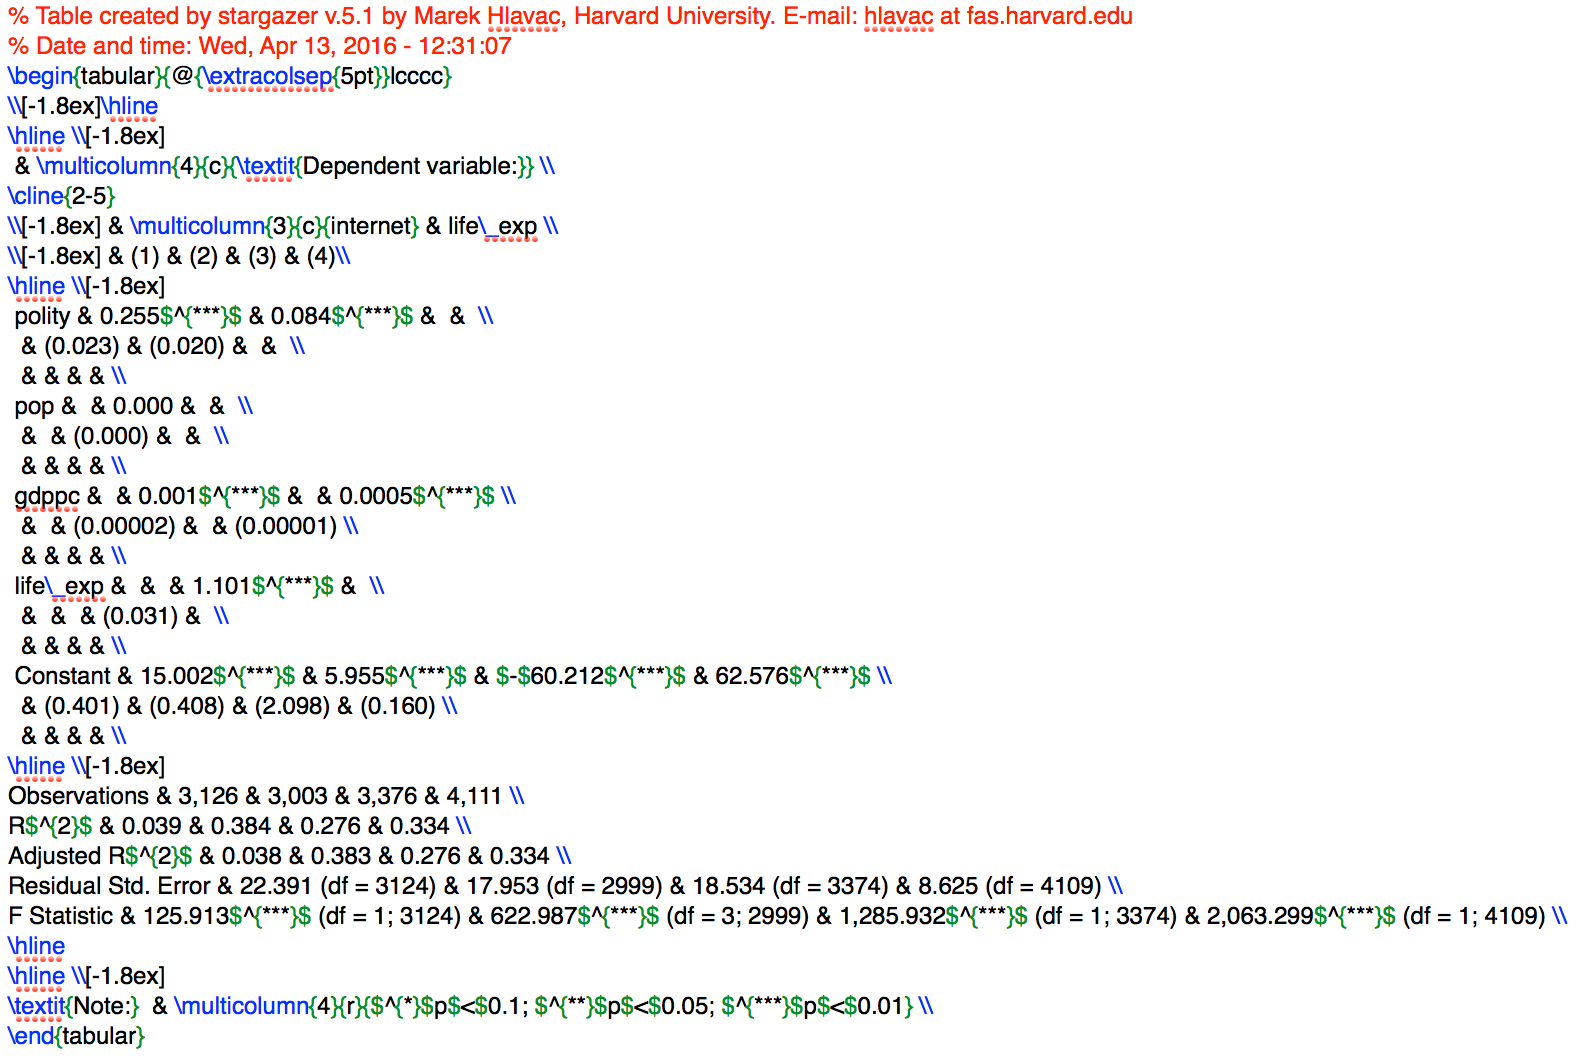
\includegraphics[width = 0.9\textwidth]{tab_simple.png}
\label{default}
\end{center}
\end{figure}
 \end{frame}
 
\begin{frame}
\frametitle{\texttt{stargazer} output with {\LaTeX} typesetting}
\resizebox{\linewidth}{!}{

% Table created by stargazer v.5.1 by Marek Hlavac, Harvard University. E-mail: hlavac at fas.harvard.edu
% Date and time: Wed, Apr 13, 2016 - 12:31:07
\begin{tabular}{@{\extracolsep{5pt}}lcccc} 
\\[-1.8ex]\hline 
\hline \\[-1.8ex] 
 & \multicolumn{4}{c}{\textit{Dependent variable:}} \\ 
\cline{2-5} 
\\[-1.8ex] & \multicolumn{3}{c}{internet} & life\_exp \\ 
\\[-1.8ex] & (1) & (2) & (3) & (4)\\ 
\hline \\[-1.8ex] 
 polity & 0.255$^{***}$ & 0.084$^{***}$ &  &  \\ 
  & (0.023) & (0.020) &  &  \\ 
  & & & & \\ 
 pop &  & 0.000 &  &  \\ 
  &  & (0.000) &  &  \\ 
  & & & & \\ 
 gdppc &  & 0.001$^{***}$ &  & 0.0005$^{***}$ \\ 
  &  & (0.00002) &  & (0.00001) \\ 
  & & & & \\ 
 life\_exp &  &  & 1.101$^{***}$ &  \\ 
  &  &  & (0.031) &  \\ 
  & & & & \\ 
 Constant & 15.002$^{***}$ & 5.955$^{***}$ & $-$60.212$^{***}$ & 62.576$^{***}$ \\ 
  & (0.401) & (0.408) & (2.098) & (0.160) \\ 
  & & & & \\ 
\hline \\[-1.8ex] 
Observations & 3,126 & 3,003 & 3,376 & 4,111 \\ 
R$^{2}$ & 0.039 & 0.384 & 0.276 & 0.334 \\ 
Adjusted R$^{2}$ & 0.038 & 0.383 & 0.276 & 0.334 \\ 
Residual Std. Error & 22.391 (df = 3124) & 17.953 (df = 2999) & 18.534 (df = 3374) & 8.625 (df = 4109) \\ 
F Statistic & 125.913$^{***}$ (df = 1; 3124) & 622.987$^{***}$ (df = 3; 2999) & 1,285.932$^{***}$ (df = 1; 3374) & 2,063.299$^{***}$ (df = 1; 4109) \\ 
\hline 
\hline \\[-1.8ex] 
\textit{Note:}  & \multicolumn{4}{r}{$^{*}$p$<$0.1; $^{**}$p$<$0.05; $^{***}$p$<$0.01} \\ 
\end{tabular} 

}
\end{frame}

\begin{frame}
\frametitle{Fancier \texttt{stargazer} output}
\resizebox{\linewidth}{!}{

% Table created by stargazer v.5.1 by Marek Hlavac, Harvard University. E-mail: hlavac at fas.harvard.edu
% Date and time: Tue, Apr 12, 2016 - 11:28:03
\begingroup 
\scriptsize 
\begin{tabular}{@{\extracolsep{0pt}}lcccc} 
\\[-1.8ex]\hline 
\hline \\[-1.8ex] 
 & \multicolumn{4}{c}{\textit{Dependent variable:}} \\ 
\cline{2-5} 
\\[-1.8ex] & \multicolumn{3}{c}{Internet Users} & Life Expectancy \\ 
\\[-1.8ex] & (1) & (2) & (3) & (4)\\ 
\hline \\[-1.8ex] 
 Polity Score & 0.2553$^{***}$ & 0.0842$^{***}$ &  &  \\ 
  & (0.0228) & (0.0202) &  &  \\ 
  Population &  & 0.0000 &  &  \\ 
  &  & (0.0000) &  &  \\ 
  GDP p.c. &  & 0.0010$^{***}$ &  & 0.0005$^{***}$ \\ 
  &  & (0.00002) &  & (0.00001) \\ 
  Life Expectancy &  &  & 1.1005$^{***}$ &  \\ 
  &  &  & (0.0307) &  \\ 
  Constant & 15.0024$^{***}$ & 5.9550$^{***}$ & $-$60.2123$^{***}$ & 62.5757$^{***}$ \\ 
  & (0.4005) & (0.4082) & (2.0975) & (0.1602) \\ 
 \hline \\[-1.8ex] 
Observations & 3,126 & 3,003 & 3,376 & 4,111 \\ 
R$^{2}$ & 0.0387 & 0.3839 & 0.2760 & 0.3343 \\ 
Adjusted R$^{2}$ & 0.0384 & 0.3833 & 0.2757 & 0.3341 \\ 
Residual Std. Error & 22.3914 (df = 3124) & 17.9527 (df = 2999) & 18.5340 (df = 3374) & 8.6253 (df = 4109) \\ 
\hline 
\hline \\[-1.8ex] 
\textit{Note:}  & \multicolumn{4}{r}{$^{*}$p$<$0.1; $^{**}$p$<$0.05; $^{***}$p$<$0.01} \\ 
\end{tabular} 
\endgroup 

}
\end{frame}
 
%%
\subsection{Math typesetting and formal presentation}
\begin{frame}[fragile=singleslide]
\frametitle{Professional typesetting of math symbols}
\begin{scriptsize}
\begin{verbatim}
\begin{equation*}
\begin{split}
\frac{\partial EU_{ns_p}}{\partial s}&=A(v)f\gamma-S'(s)\leq0\\
\frac{\partial^2 EU_{ns_p}}{\partial s^2}&=-S''(s)<0
\end{split}
\end{equation*}\end{verbatim}
\end{scriptsize}
\begin{equation*}
\begin{split}
\frac{\partial EU_{ns_p}}{\partial s}&=A(v)f\gamma-S'(s)\leq0\\
\frac{\partial^2 EU_{ns_p}}{\partial s^2}&=-S''(s)<0
\end{split}
\end{equation*}
\end{frame}
 
\begin{frame}[fragile=singleslide]
\frametitle{Professional typesetting of regression equations}
\begin{scriptsize}
\begin{verbatim}
\begin{equation*}
\text{exp}_{i,t} = \beta_1\text{conflict}_{i,t-1} + 
	\beta_2\text{coca}_{i,t-1} + 
	\beta_3\text{conflict}_{i,t-1} \times \text{coca}_{i,t-1} 
	+ c_i + \delta_t + \epsilon_{i,t}
\end{equation*}
\end{verbatim}
\begin{equation*}
\text{exp}_{i,t} = \beta_1\text{conflict}_{i,t-1} + 
\beta_2\text{coca}_{i,t-1} + 
\beta_3\text{conflict}_{i,t-1}\times\text{coca}_{i,t-1} +c_i+\delta_t+\epsilon_{i,t}
\end{equation*}
\end{scriptsize}
\end{frame}
 
\begin{frame}
\frametitle{Professional math typesetting}
\begin{block}{Basic list of math symbols in {\LaTeX}}%
	\url{http://web.ift.uib.no/Teori/KURS/WRK/TeX/symALL.html}
\end{block}
\end{frame}

\begin{frame}
\frametitle{Game trees with \texttt{tikz} package}
\begin{center}
\usetikzlibrary{calc}
  \tikzset{
    % Two node styles for game trees: solid and hollow
    solid node/.style={circle,draw,inner sep=1.5,fill=black},
    hollow node/.style={circle,draw,inner sep=1.5}
}
\begin{tikzpicture}[scale=1.2,font=\scriptsize]
  % Specify spacing for each level of the tree
    \tikzstyle{level 1}=[level distance=15mm,sibling distance=35mm]
    \tikzstyle{level 2}=[level distance=15mm,sibling distance=15mm]
  % The Tree
  \node(0)[hollow node,label=above:{State 1}]{}
    child{node(1)[hollow node]{}
      child{node[solid node,label=below:{$(1-c,-k)$}]{} edge from parent node[left]{$s$}}
      child{node[solid node,label=below:{$(1,0)$}]{} edge from parent node[right]{$n$}}
      edge from parent node[left,xshift=-3]{$v$}
    }
    child{node(2)[hollow node]{}
      child{node[solid node,label=below:{$(-c,1-k)$}]{} edge from parent node[left]{$s$}}
      child{node[solid node,label=below:{$(0,1)$}]{} edge from parent node[right]{$n$}}
      edge from parent node[right,xshift=3]{$n$}
};
  \node at ($(1)!.5!(2)$) {US};
\end{tikzpicture}
\end{center}
\end{frame}


\begin{frame}[fragile]
\frametitle{Game trees with \texttt{tikz} package}
\begin{Verbatim}[fontsize=\tiny]
\usetikzlibrary{calc}
  \tikzset{
    solid node/.style={circle,draw,inner sep=1.5,fill=black},
    hollow node/.style={circle,draw,inner sep=1.5}
}
\begin{tikzpicture}[scale=1.2,font=\scriptsize]
    \tikzstyle{level 1}=[level distance=15mm,sibling distance=35mm]
    \tikzstyle{level 2}=[level distance=15mm,sibling distance=15mm]
  \node(0)[hollow node,label=above:{State 1}]{}
    child{node(1)[hollow node]{}
      child{node[solid node,label=below:{$(1-c,-k)$}]{} edge from parent node[left]{$s$}}
      child{node[solid node,label=below:{$(1,0)$}]{} edge from parent node[right]{$n$}}
      edge from parent node[left,xshift=-3]{$v$}
    }
    child{node(2)[hollow node]{}
      child{node[solid node,label=below:{$(-c,1-k)$}]{} edge from parent node[left]{$s$}}
      child{node[solid node,label=below:{$(0,1)$}]{} edge from parent node[right]{$n$}}
      edge from parent node[right,xshift=3]{$n$}
};
  \node at ($(1)!.5!(2)$) {US};
\end{tikzpicture}
\end{Verbatim}
\end{frame}

\begin{frame}
\frametitle{Diagrams with \texttt{tikz} package}
\usetikzlibrary{arrows.meta, shapes}
\centering
\tikzstyle{hv}=[circle,draw]
\tikzstyle{ovt}=[hv,fill=blue!10]
\tikzstyle{ovc}=[hv,fill=black!10]
\tikzstyle{a}=[-{Latex[length=2mm,width=1.5mm]}]
\tikzstyle{ao}=[a,dashed]
\tikzstyle{across}=[a,red]
\tikzstyle{d}=[above]
\tikzstyle{both}=[{Latex[length=2mm,width=1.5mm]}-{Latex[length=2mm,width=1.5mm]},red]

\begin{tikzpicture}[every node/.style={scale=1}]
  \node (z11) at (-3,2) [hv] {\(z_{1,1}\)};
  \node (z12) at (0,2) [hv] {\(z_{1,2}\)};
  \node (z1n) at (4,2) [hv] {\(z_{R,N}\)};
  \node (y11t) at (-3.75,3.5) [ovt] {\scriptsize\(y^{(T)}_{1,1}\)};
  \node (y11c) at (-2.25,3.5) [ovc] {\scriptsize\(y^{(C)}_{1,1}\)};
  \node (y12t) at (-0.75,3.5) [ovt] {\scriptsize\(y^{(T)}_{1,2}\)};
  \node (y12c) at (0.75,3.5) [ovc] {\scriptsize\(y^{(C)}_{1,2}\)};
  \node (y1nt) at (3.25,3.5) [ovt] {\scriptsize\(y^{(T)}_{R,N}\)};
  \node (y1nc) at (4.75,3.5) [ovc] {\scriptsize\(y^{(C)}_{R,N}\)};
  \node (z1dots) at (2,2) {\ldots};
  \draw[a] (z11) -- (z12);
  \draw[a] (z12) -- (z1dots);
  \draw[a] (z1dots) -- (z1n);
  \draw[ao] (z11) -- (y11t);
  \draw[ao] (z11) -- (y11c);
  \draw[ao] (z12) -- (y12t);
  \draw[ao] (z12) -- (y12c);
  \draw[ao] (z1n) -- (y1nt);
  \draw[ao] (z1n) -- (y1nc);

  \node (z21) at (-3,0) [hv] {\(z_{2,1}\)};
  \node (z22) at (0,0) [hv] {\(z_{2,2}\)};
  \node (z2n) at (4,0) [hv] {\(z_{R,N}\)};
  \node (y21t) at (-3.75,-1.5) [ovt] {\scriptsize\(y^{(T)}_{2,1}\)};
  \node (y21c) at (-2.25,-1.5) [ovc] {\scriptsize\(y^{(C)}_{2,1}\)};
  \node (y22t) at (-0.75,-1.5) [ovt] {\scriptsize\(y^{(T)}_{2,2}\)};
  \node (y22c) at (0.75,-1.5) [ovc] {\scriptsize\(y^{(C)}_{2,2}\)};
  \node (y2nt) at (3.25,-1.5) [ovt] {\scriptsize\(y^{(T)}_{R,N}\)};
  \node (y2nc) at (4.75,-1.5) [ovc] {\scriptsize\(y^{(C)}_{R,N}\)};
  \node (z2dots) at (2,0) {\ldots};
  \draw[a] (z21) -- (z22);
  \draw[a] (z22) -- (z2dots);
  \draw[a] (z2dots) -- (z2n);
  \draw[ao] (z21) -- (y21t);
  \draw[ao] (z21) -- (y21c);
  \draw[ao] (z22) -- (y22t);
  \draw[ao] (z22) -- (y22c);
  \draw[ao] (z2n) -- (y2nt);
  \draw[ao] (z2n) -- (y2nc);

  \draw[across] (z11) -- (z22);
  \draw[across] (z21) -- (z12);
  \draw[across] (z22) -- (z1dots);
  \draw[across] (z12) -- (z2dots);
  \draw[across] (z1dots) -- (z2n);
  \draw[across] (z2dots) -- (z1n);
  
 \draw[both] (z11) -- (z21);
 \draw[both] (z12) -- (z22);
 \draw[both] (z1dots) -- (z2dots);
 \draw[both] (z1n) -- (z2n);

\end{tikzpicture}
\end{frame}


\begin{frame}[fragile]
\frametitle{Diagrams with \texttt{tikz} package}
\begin{Verbatim}[fontsize=\tiny]
\tikzstyle{hv}=[circle,draw]
\tikzstyle{ovt}=[hv,fill=blue!10]
\tikzstyle{ovc}=[hv,fill=black!10]
\tikzstyle{a}=[-{Latex[length=2mm,width=1.5mm]}]
\tikzstyle{ao}=[a,dashed]
\tikzstyle{across}=[a,red]
\tikzstyle{d}=[above]
\tikzstyle{both}=[{Latex[length=2mm,width=1.5mm]}-{Latex[length=2mm,width=1.5mm]},red]
\begin{tikzpicture}[every node/.style={scale=1}]
  \node (z11) at (-3,2) [hv] {\(z_{1,1}\)};
  \node (z12) at (0,2) [hv] {\(z_{1,2}\)};
  \node (z1n) at (4,2) [hv] {\(z_{R,N}\)};
  \node (y11t) at (-3.75,3.5) [ovt] {\scriptsize\(y^{(T)}_{1,1}\)};
  \node (y11c) at (-2.25,3.5) [ovc] {\scriptsize\(y^{(C)}_{1,1}\)};
  \node (y12t) at (-0.75,3.5) [ovt] {\scriptsize\(y^{(T)}_{1,2}\)};
  \node (y12c) at (0.75,3.5) [ovc] {\scriptsize\(y^{(C)}_{1,2}\)};
  \node (y1nt) at (3.25,3.5) [ovt] {\scriptsize\(y^{(T)}_{R,N}\)};
  \node (y1nc) at (4.75,3.5) [ovc] {\scriptsize\(y^{(C)}_{R,N}\)};
  \node (z1dots) at (2,2) {\ldots};
  \draw[a] (z11) -- (z12);
  \draw[a] (z12) -- (z1dots);
  \draw[a] (z1dots) -- (z1n);
  \draw[ao] (z11) -- (y11t);
  \draw[ao] (z11) -- (y11c);
  \draw[ao] (z12) -- (y12t);
  ...
\end{tikzpicture}
\end{Verbatim}
\end{frame}
 
 %%% CHALLENGES
 \section{Challenges}\label{challenge}
 
 %%
 \subsection{Steep Learning Curve}
 
\begin{frame}
\frametitle{Steep Learning Curve}
\begin{block}{The key to learning {\LaTeX}}
\begin{itemize}
\item Learning by doing
\item Trial and error
\item Google
\item \textsc{PATIENCE}
\end{itemize}
 \end{block}
\end{frame}
 
 %%
\subsection{Collaboration and journal submission}

\begin{frame}
\frametitle{Co-Authoring}
Reproducibility is one of the main advantages of {\LaTeX}. But co-authoring can be tricky with a basic {\LaTeX} distribution.
\begin{block}{Challenges toward collaboration}%
\begin{itemize}
\item Co-authors that don't know {\LaTeX}.
\item Special packages, fonts, etc. 
\item Limited tracking of changes.
\item Limited commenting abilities (except \texttt{\%} or ).
\end{itemize}
\end{block}
\end{frame} 
 
\begin{frame}
\frametitle{Tools for collaboration}
 \begin{block}{Online platform \url{https://www.overleaf.com}}%
Limited free version, many templates.
\end{block}
\begin{block}{\texttt{todonotes} package}
Adds margin and in-text comments.
\end{block}
\end{frame}


\begin{frame}
\frametitle{Journal submission}
\begin{itemize}
\item Some journals will not accept {\LaTeX} files for final manuscript submission. 
\item There are software tools for converting {\LaTeX} to Word, but it is a \underline{pain}.
\item Especially frustrating for: Tables, bibliographies, equations. Hence, all the reasons why you would want to use {\LaTeX} in the first place.
\end{itemize}
\end{frame}

%% 
\subsection{Miscellaneous}

\begin{frame}
\frametitle{Other Challenges}
\begin{itemize}
\item Limited spell-checking options. Depends on editor.
\item Debugging is part of the process.
\begin{itemize}
\item Check for typos.
\item Read error message of compiler.
\item Google error message.
\item Trial and error.
\end{itemize}
\end{itemize}
\end{frame}
 
\begin{frame}
\frametitle{Some misconceptions}
\begin{block}{No word counts}%
Many compilers don't have a build in function, but there is external programs (e.g. \url{http://app.uio.no/ifi/texcount/}) and ShareLaTeX also has a word count option.
\end{block}
\begin{block}{Tables in {\LaTeX} suck}%
Programming tables from scratch is no fun! But, there are tools such as the \texttt{stargazer} and \texttt{estout} packages, plug-ins for Excel, and online tools (\url{http://www.tablesgenerator.com}).
\end{block}
\end{frame} 
 
%%% STRUCTURE
\section{Structure and compiling}\label{structure}

%%
\subsection{Structure of a {\LaTeX} document}

\begin{frame}[fragile=singleslide]
\frametitle{Basic Structure}
\begin{block}{Preamble}%
Document type, basic settings, packages. Not printed.
\end{block}
\begin{block}{Title section}%
Title, date, author information.
\end{block}
\begin{block}{Main Body}%
Document content including title wrapped by \begin{verbatim}\being{document} ... \end{document}.\end{verbatim}
\end{block}
\end{frame}

\begin{frame}
\frametitle{Preamble}
\begin{columns}[T]%
\begin{column}{.7\textwidth}
\begin{figure}[h!] 
\begin{center}
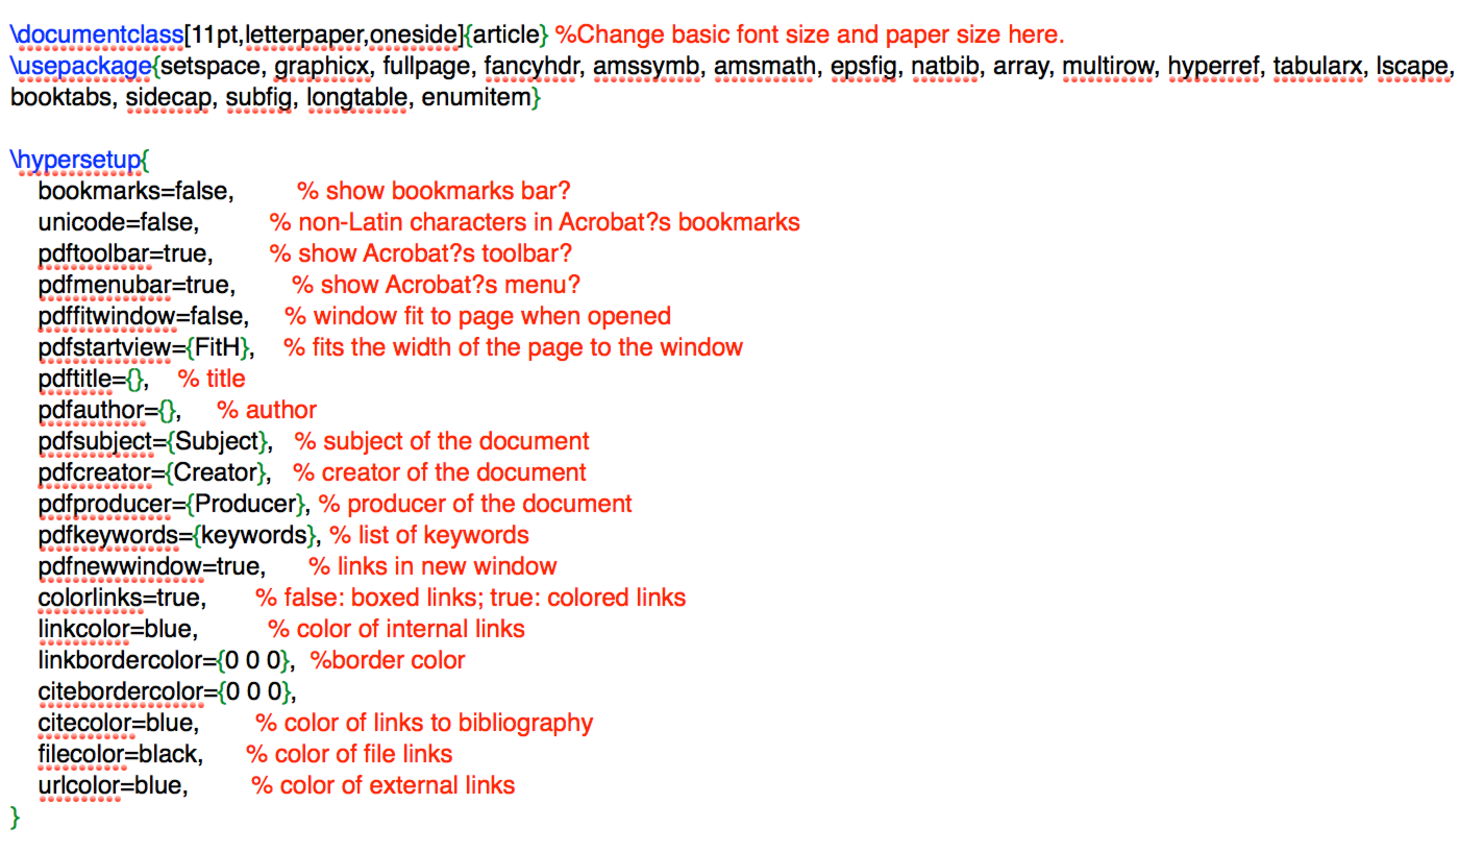
\includegraphics[width = 3.3in]{preamble.pdf}
\end{center}
\end{figure}
\end{column}%
\hfill
\begin{column}{.3\textwidth}
Most important parameter is \texttt{\\documentclass\{\}}
\begin{itemize}
\item article
\item resume
\item beamer
\item letter
\end{itemize}
Packages and hypersetup differ.
\end{column}%
\end{columns}
\end{frame}

%%
\subsection{Compiling documents}

\begin{frame}
\frametitle{Compiling a document}
 Workflow might differ for each editor. Example TeXShop:
\begin{enumerate}
\item Running {\LaTeX} first time will produce general text.
\item Running BibTeX to create bibliography (if necessary).
\item Running {\LaTeX} second time will product internal links, table of contents, and references.
\end{enumerate}
Some editors like Overleaf will compile everything at once.
\end{frame}

\begin{frame}[fragile=singleslide]
\frametitle{{\LaTeX} commands and special characters}
All {\LaTeX} commands start with a \texttt{\textbackslash}. Example: \texttt{\textbackslash begin\{\}}
\begin{block}{Characters with special meaning}
\begin{itemize}
\item \texttt{\{} and \texttt{\}}: Used in functions and for delineation.
\item \texttt{\%}: Comment (nothing that follows will be printed).
\item \texttt{\$}: In-line math.
\item \texttt{\&}: Alignment character (tables and math).
\end{itemize}
\end{block}
To use any of these symbols in text, we need to use an escape character. For example, to print \% \& \$, we need to type:
\begin{verbatim}
\% \& \$
\end{verbatim}
\end{frame}

\begin{frame}
\frametitle{Miscellaneous Notes}
\begin{itemize}
\item<1-> Using \texttt{section\{\}}, \texttt{subsection\{\}}, and \texttt{subsubsection\{\}}, {\LaTeX} automatically creates a structure that pdf readers will understand.
\item<2-> \texttt{section*\{\}}, \texttt{subsection*\{\}}, and \texttt{subsubsection*\{\}} are the non-numbered equivalents.
\item<3-> Size of headings will automatically be chosen by  {\LaTeX}.
\item<4-> White space typically does not matter.
\item<5-> Create internal links using \texttt{label\{\}} and \texttt{ref\{\}}.
\item<6-> Citations can automatically be included as internal links.
\end{itemize}
\end{frame}

\section{Bibliographies}\label{bib}
\begin{frame}[fragile]
\frametitle{Basic structure}
\begin{block}{Bibliographic data base, e.g. \texttt{sample\_bib.bib}.}
\begin{Verbatim}[fontsize=\scriptsize]
@article{fearonlaitin2003,
	Author = {James D. Fearon and David D. Laitin},
	Journal = {American Political Science Review},
	Number = {1},
	Pages = {75-90},
	Title = {{Ethnicity, Insurgency, and Civil War}},
	Volume = {97},
	Year = {2003}}
\end{Verbatim}
\end{block}\pause
\begin{block}{Building bibliography within to \texttt{.tex} document}
\begin{Verbatim}[fontsize=\footnotesize]
\bibliographystyle{chicago}
\bibliography{sample_bib.bib}
\end{Verbatim}
\end{block}\pause
\begin{block}{Citations}
\begin{Verbatim}[fontsize=\footnotesize]
\citep{fearonlaitin2003}
\end{Verbatim}
\end{block}
\end{frame}

\begin{frame}
\frametitle{Notes on bibliographies}
\begin{itemize}
\item<1-> Use a citation manager to create/manage .bib file.
\begin{itemize}
\item<2-> Personally use BibDesk, but there are many others.
\item<3-> Bibliographic data, notes, PDFs, etc, in one place.
\item<4-> Use keywords or tags for organization.
\item<5-> Have one master .bib file and reference it in each .tex document.
\end{itemize}
\item<6-> Overleaf offers integration with Zotero and Mendeley.
\item<7-> Easy switching between citation styles.
\end{itemize}
\end{frame}


\begin{frame}
\frametitle{Some aspects we did not cover today}
\begin{itemize}
\item<1-> Special document types such as \texttt{beamer} for presentations, letters, and resumes.
\item<2-> XeTeX and XeLaTeX (special engines).
\item<3-> Style files (think: templates for .ppt).
\item<4-> Technical background for {\LaTeX} and {\TeX} programming language. 
\end{itemize}
\end{frame}



\begin{frame}
\frametitle{Moving on...}
\Large
Any questions before we move on to part II?
\end{frame}

\begin{frame}
\frametitle{{\LaTeX} Lingo}
\begin{block}{Distribution}%
Collection of {\TeX}-related software. Examples: MiKTeX, TeX Live.
\end{block}
\begin{block}{Editor}%
Creation of documents. Examples: TeXworks, TeXShop.
\end{block}
\begin{block}{Format}%
Different {\TeX}-based languages. Examples: {\LaTeX}, plain {\TeX}.
\end{block}
\begin{block}{Packages}%
Add ons to basic systems. Examples graphicx, natbib.
\end{block}
\end{frame}

\end{document}
%% EOF

